% ============================================================
% M2 轮4 S3 · 练习件 第6课时（§1.2.1 空间中的点、直线与空间向量）
% 题面：照题面库 成卷/题面库/课时06-1.2.1.md 全 16 题冻结入卷（卷面题号＝库序 1~16）；
%       组名/难度照库头第 3/4 字段（〔代表〕〔第2题〕簿记标不入版面，同批1口径；「复用库名」注记照登）。
%       第9/16题（教材题）库面「如图」而库无【图】位＝S1 冻结态：长方体以顶点命名自足、图无信息增量，
%       照登不配图（同批1课时01「图依赖已文字化」口径），登记呈。
%       【装配轮0912】已删题9/16「如图（所示），」语销债（题面自足、删语后无悬空指代；同拓册批6「有言无图删语」先例）。
%       第10题清稿注（补「正方形对角线互相平分」句＋知识点重标）＝详解侧，答案册轮执行；题面照登。
%       全卷 v1/v2 等下标脱字（库面「v2」）按亲算/讲部原式规范化为 \(v_2\)（记号归一，改字不改果，落台账）。
% 模板基线＝练习线样张（六宏零改动拷入）；版式＝练习线 p2 课时训练
%       （\keshi＋multicols＋花形三档 基础巩固1~10／综合提升11~14／思维探索15~16）。
% 图源：第10题＝单元5 image2.png→dy5_image2.png(34mm，F5·7 正方体图，源位图逐字节 cmp)；
%       第11题＝讲上 image13.png→js_image13.png(30mm)；第12题＝讲上 image14.png→js_image14.png(40mm)；
%       第14题＝讲上 image17.png→js_image17.png(24mm)；第15题＝讲上 image37.png→js_image37.png(30mm，曲池渲染图)。
%       （js_* 与导学件课时06 figs 逐字节一致，后者经批3 与讲上 docx media cmp 核验。）
% 取值/组名照登对照/图位/登记事项：见 ../批2值台账.md 课时06 节。
% 编译：xelatex main.tex（两遍）→ python render.py → png/pageN.png
% ============================================================
\documentclass[fontset=none]{ctexart}
\usepackage{qp-m3} % 换装：六宏→qp-m3 单包（钉后版 md5 7c3930362be8a0a2bdf21bbf8ac16573，两补钉随版）

% ============================================================
% 练习件局部宏（照练习线样张页2形制搬入；本段只加件，不改件）
% ============================================================
\renewcommand{\qpjianming}{练习件}
\renewcommand{\qpceming}{高中数学\quad 选择性必修第一册(人教B版)} % 换装回钉：qp-m3 默认册名＝选必二，防页脚漂移（试迁规约·试迁报告§四 B3 实证必改）
\renewcommand{\qpzhangming}{第一章\quad 空间向量与立体几何}

% ---------- YJ-01 灰块页脚·练习册档（块 31.0×7.8mm，照练习线样张 31.0mm 修正版） ----------
\newcommand{\qpxsyema}{\ifnum\value{page}<10 00\fi\ifnum\value{page}>9 \ifnum\value{page}<100 0\fi\fi\arabic{page}}
\newcommand{\lxshuziL}{\hbox to 13.8mm{\setlength{\fboxsep}{0pt}\colorbox{pnumbg}{%
  \makebox[31.0mm][l]{\rule[-3.145mm]{0pt}{7.8mm}\hspace{2.8mm}\fontsize{10.7pt}{13pt}\selectfont\color{black}\numpnum\qpxsyema}}\hss}}
\newcommand{\lxshuziR}{\hbox to 13.8mm{\kern-17.2mm\setlength{\fboxsep}{0pt}\colorbox{pnumbg}{%
  \makebox[31.0mm][r]{\rule[-3.145mm]{0pt}{7.8mm}\fontsize{10.7pt}{13pt}\selectfont\color{black}\numpnum\qpxsyema\hspace{2.75mm}}}}}
\fancyfoot[RO]{\raisebox{-1.24mm}[0pt][0pt]{\qphuitext\qpzhangming\quad{\heiti\qpjianming}\hspace{3mm}\lxshuziL}}
\fancyfoot[LE]{\raisebox{-1.24mm}[0pt][0pt]{\lxshuziR\hspace{3mm}\qphuitext\qpceming}}

% ---------- HX-01 花形·三档名（练习册版 25.5×6.8mm，重叠 o＝5.1mm，照练习线样张裁定值） ----------
% 局部宏 \huadianOverlapLx 已由 qp-m3 收编（等值定义），依换装方案§1.4 预删防撞名
% 局部宏 \dangbadge 已由 qp-m3 收编（等值定义），依换装方案§1.4 预删防撞名

% ---------- TJ-02 练习册悬挂题号（单号 5.75mm／双位 7.6mm，题号 \textbf 加重） ----------
% 长度 \lxhang 已由 qp-m3 分配，预删防重复定义
% 局部宏 \tihao 已由 qp-m3 收编（等值定义），依换装方案§1.4 预删防撞名
% 选项段（TJ-07 行距档；左缘随题号悬挂）
% 局部宏 \lxopt 已由 qp-m3 收编（等值定义），依换装方案§1.4 预删防撞名
% 解答题书写位留白
% 局部宏 \xiexwei 已由 qp-m3 收编（等值定义），依换装方案§1.4 预删防撞名
% 组名栏宏（组名照题面库头第 3 字段照登，去〔代表〕〔第N题〕簿记标）
% 局部宏 \zu 已由 qp-m3 收编（等值定义），依换装方案§1.4 预删防撞名

\begin{document}
%成书重装五本跨本连续页码（G7方案B，承M2/M3装配先例）setcounter 注入位
\setcounter{page}{66}

% ============================================================
% 课时训练（三档 10＋4＋2＝16 题）
% ============================================================
\keshi{第6课时\quad 空间中的点、直线与空间向量}
\begin{multicols}{2}
\emergencystretch=1em

\dangbadge{基}{础}{巩}{固}

\tihao{1}\zu{K1 直线的方向向量·概念辨析×选择} \tieside{简单}若\(A(-1,0,2)\)，\(B(1,4,10)\)在直线\(l\)上，则直线\(l\)的一个方向向量为\nobreak(\kongwei)
\lxopt{\makebox[\dimexpr0.25\linewidth-0.25\lxhang-0.25em\relax][l]{A．\((1,2,4)\)；}\makebox[\dimexpr0.25\linewidth-0.25\lxhang-0.25em\relax][l]{B．\((1,4,2)\)；}\makebox[\dimexpr0.25\linewidth-0.25\lxhang-0.25em\relax][l]{C．\((2,1,4)\)；}\makebox[\dimexpr0.25\linewidth-0.25\lxhang-0.25em\relax][l]{D．\((4,2,1)\)}}
\begin{ansblock}[练-课时06-1]
% ans:练-课时06-1
\ansitem{1}{A}
\end{ansblock}

\tihao{2}\zu{K1 开放填空写出方向向量} \tieside{简单}设\((2,-2,1)\)，\((3,-3,1)\)是空间直线\(l\)上的点，求直线\(l\)的一个方向向量．
\xiexwei{16mm}
\begin{ansblock}[练-课时06-2]
% ans:练-课时06-2
\ansitem{2}{\((1,-1,0)\) 的任一非零倍数}
\end{ansblock}

\tihao{3}\zu{K2 方向向量判两线位置·判断题组} \tieside{简单}设\(\overrightarrow{v_1}\)，\(\overrightarrow{v_2}\)分别是空间中两条不重合的直线\(l_1\)，\(l_2\)的方向向量，分别根据下列条件判断直线\(l_1\)，\(l_2\)的位置关系：
\lxopt{(1)\(\overrightarrow{v_1}=(0,0,1)\)，\(\overrightarrow{v_2}=(0,0,-3)\)；}
\lxopt{(2)\(\overrightarrow{v_1}=(2,-1,-2)\)，\(\overrightarrow{v_2}=(6,-3,-6)\)．}
\xiexwei{16mm}
\begin{ansblock}[练-课时06-3]
% ans:练-课时06-3
\ansitem{3}{(1)(2) 均平行}
\end{ansblock}

\tihao{4}\zu{K3 线线位置·平行\(\Rightarrow\)共线求参} \tieside{简单}\(l_1\)的方向向量为\(\overrightarrow{v_1}=(1,2,3)\)，\(l_2\)的方向向量\(\overrightarrow{v_2}=(\lambda,4,6)\)，若\(l_1\parallel l_2\)，则\(\lambda\)等于\nobreak(\kongwei)
\lxopt{\makebox[\dimexpr0.25\linewidth-0.25\lxhang-0.25em\relax][l]{A．\(1\)；}\makebox[\dimexpr0.25\linewidth-0.25\lxhang-0.25em\relax][l]{B．\(2\)；}\makebox[\dimexpr0.25\linewidth-0.25\lxhang-0.25em\relax][l]{C．\(3\)；}\makebox[\dimexpr0.25\linewidth-0.25\lxhang-0.25em\relax][l]{D．\(4\)}}
\begin{ansblock}[练-课时06-4]
% ans:练-课时06-4
\ansitem{4}{B（\(\lambda=2\)）}
\end{ansblock}

\tihao{5}\zu{K3 垂直\(\Rightarrow\)点积零} \tieside{简单}设直线\(l_1\)，\(l_2\)的方向向量分别为\(\overrightarrow{a}=(1,2,-2)\)，\(\overrightarrow{b}=(-2,3,m)\)，若\(l_1\perp l_2\)，则实数\(m\)等于\nobreak(\kongwei)
\lxopt{\makebox[\dimexpr0.25\linewidth-0.25\lxhang-0.25em\relax][l]{A．\(1\)；}\makebox[\dimexpr0.25\linewidth-0.25\lxhang-0.25em\relax][l]{B．\(2\)；}\makebox[\dimexpr0.25\linewidth-0.25\lxhang-0.25em\relax][l]{C．\(3\)；}\makebox[\dimexpr0.25\linewidth-0.25\lxhang-0.25em\relax][l]{D．\(4\)}}
\begin{ansblock}[练-课时06-5]
% ans:练-课时06-5
\ansitem{5}{B（\(m=2\)）}
\end{ansblock}

\tihao{6}\zu{K4 求点坐标·向量等式正向} \tieside{简单}已知点\(A(3,4,5)\)，\(B(3,4,0)\)，\(\overrightarrow{BC}=2\overrightarrow{OA}\)，且\(O\)为坐标原点，求点\(C\)的坐标．
\xiexwei{16mm}
\begin{ansblock}[练-课时06-6]
% ans:练-课时06-6
\ansitem{6}{C\((9,12,10)\)}
\end{ansblock}

\tihao{7}\zu{K4 双垂直方程组逆向反求} \tieside{简单}已知点\(A(0,1,0)\)，\(B(-1,0,-1)\)，\(C(2,1,1)\)，点\(P(x,0,z)\)，若\(PA\perp\)平面\(ABC\)，则点\(P\)的坐标为\nobreak(\kongwei)
\lxopt{\makebox[\dimexpr0.5\linewidth-0.5\lxhang-0.25em\relax][l]{A．\((1,0,-2)\)；}\makebox[\dimexpr0.5\linewidth-0.5\lxhang-0.25em\relax][l]{B．\((1,0,2)\)}}
\lxopt{\makebox[\dimexpr0.5\linewidth-0.5\lxhang-0.25em\relax][l]{C．\((-1,0,2)\)；}\makebox[\dimexpr0.5\linewidth-0.5\lxhang-0.25em\relax][l]{D．\((2,0,-1)\)}}
\begin{ansblock}[练-课时06-7]
% ans:练-课时06-7
\ansitem{7}{C\((-1,0,2)\)}
\end{ansblock}

\tihao{8}\zu{K5 两线所成角·垂直特例直判} \tieside{简单}设\(\overrightarrow{v_1}=(1,2,-2)\)，\(\overrightarrow{v_2}=(-2,3,2)\)分别是空间中直线\(l_1\)，\(l_2\)的方向向量，求直线\(l_1\)，\(l_2\)所成角的大小．
\xiexwei{16mm}
\begin{ansblock}[练-课时06-8]
% ans:练-课时06-8
\ansitem{8}{\(90^{\circ}\)}
\end{ansblock}

\tihao{9}\zu{K6 异面直线所成角·标准建系直算（复用库名）} \tieside{简单}在长方体\(ABCD\text{-}\penalty100 A'B'C'D'\)中：
\lxopt{(1)哪些棱所在直线与直线\(AA'\)互为异面直线且互相垂直？}
\lxopt{(2)若\(AB=\sqrt{3}\)，\(AA'=1\)，求向量\(\overrightarrow{BA'}\)分别与\(\overrightarrow{CC'}\)，\(\overrightarrow{D'C'}\)，\(\overrightarrow{B'C'}\)的夹角．}
\xiexwei{16mm}
\begin{ansblock}[练-课时06-9]
% ans:练-课时06-9
\ansitem{9}{(1)\(BC\)、\(CD\)、\(B^{\prime}C^{\prime}\)、\(C^{\prime}D^{\prime}\)；(2)\(60^{\circ}\)／\(150^{\circ}\)／\(90^{\circ}\)}
\end{ansblock}

\tihao{10}\zu{K9 线线平行证明·中点中位线} \tieside{简单}如图，在正方体\(ABCD\text{-}\penalty100 A_1B_1C_1D_1\)中，棱长为\(2\)，\(M\)，\(N\)分别为\(A_1B\)，\(AC\)的中点，求证：\(MN\parallel B_1C\)．
\par\vspace{1.9mm}\penalty10000\noindent\makebox[\linewidth][c]{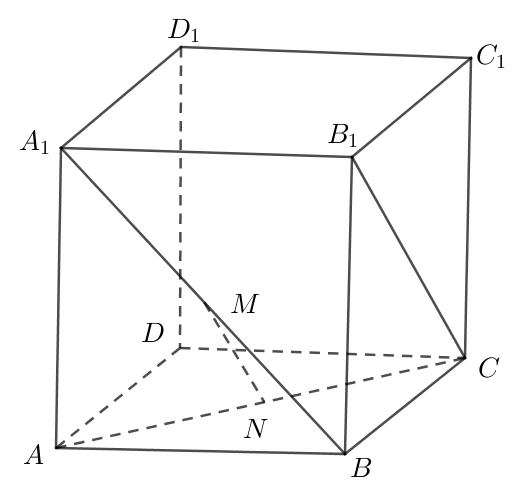
\includegraphics[width=34mm]{figs/dy5_image2.png}}\par\vspace{-1.0mm}\penalty-50
\xiexwei{16mm}
\begin{ansblock}[练-课时06-10]
% ans:练-课时06-10
\setlength{\anshang}{7.6mm}% 题10 起双位档（照答案册同值，块内局部）
\ansitem{10}{证明见解析（\(\overrightarrow{MN}=\dfrac{1}{2}\overrightarrow{B_{1}C}\)）}
\ansnote{解析}{正方形对角线互相平分——中点 \(M\)、\(N\) 为对角线交点链。}
\end{ansblock}

\dangbadge{综}{合}{提}{升}

\tihao{11}\zu{K10 向量法证线面平行＋线面垂直（双问门面）} \tieside{中档}如图，在四棱锥\(P\text{-}\penalty100 ABCD\)中，底面\(ABCD\)是正方形，侧面\(PAD\perp\)底面\(ABCD\)，且\(PA=PD=\frac{\sqrt{2}}{2}AD\)，若\(E\)、\(F\)分别为\(PC\)、\(BD\)的中点．求证：
\par\vspace{1.9mm}\penalty10000\noindent\makebox[\linewidth][c]{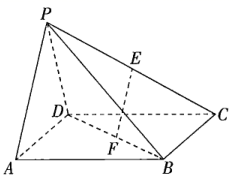
\includegraphics[width=30mm]{figs/js_image13.png}}\par\vspace{-1.0mm}\penalty10000
\lxopt{(1)\(EF\parallel\)平面\(PAD\)；}
\lxopt{(2)\(EF\perp\)平面\(PDC\)．（用向量方法证明）}
\xiexwei{16mm}
\begin{ansblock}[练-课时06-11]
% ans:练-课时06-11
\setlength{\anshang}{7.6mm}% 题11 起双位档（照答案册同值，块内局部）
\ansitem{11}{(1)(2) 证明见解析}
\end{ansblock}

\tihao{12}\zu{K7 异面直线所成角·构造垂足建系（复用库名）} \tieside{中档}如图，在三棱锥\(P\text{-}\penalty100 ABC\)中，\(\triangle ABC\)为等边三角形，\(\triangle PAC\)为等腰直角三角形，\(PA=PC=4\)，平面\(PAC\perp\)平面\(ABC\)，\(D\)为\(AB\)的中点，则异面直线\(AC\)与\(PD\)所成角的余弦值为\nobreak(\kongwei)
\par\vspace{1.9mm}\penalty10000\noindent\makebox[\linewidth][c]{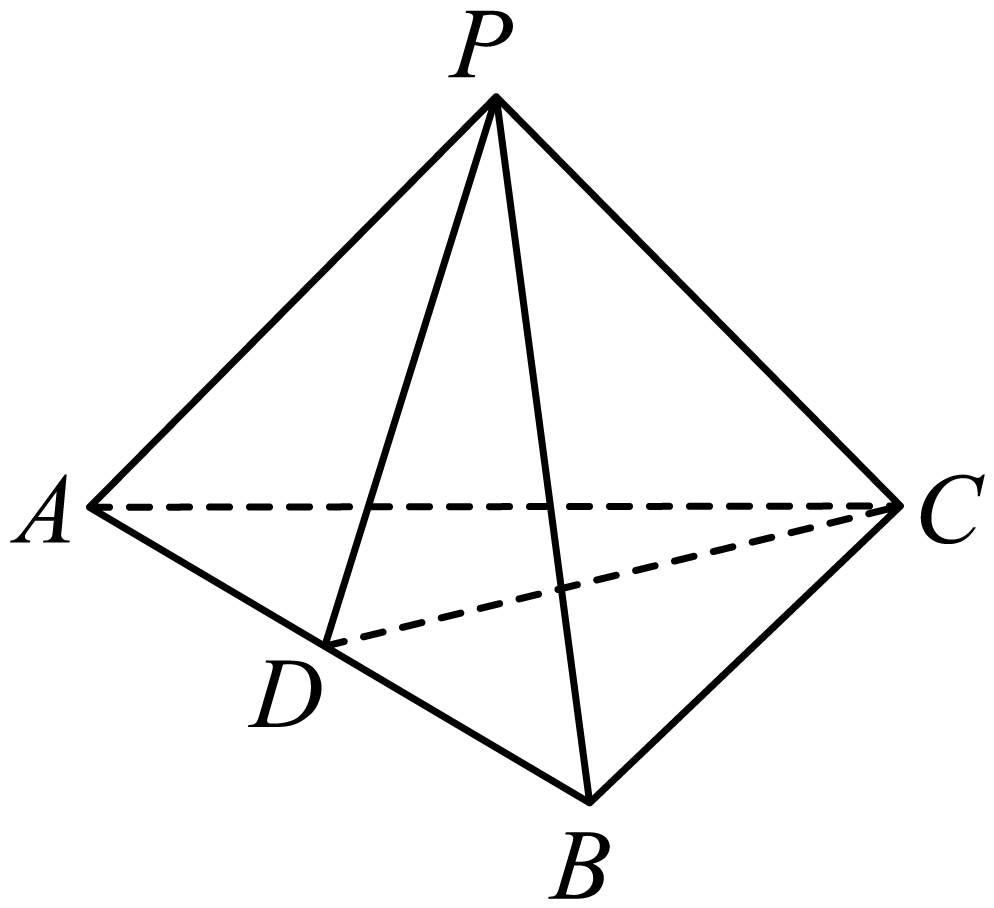
\includegraphics[width=40mm]{figs/js_image14.png}}\par\vspace{-1.0mm}\penalty10000
\lxopt{\makebox[\dimexpr0.5\linewidth-0.5\lxhang-0.25em\relax][l]{A．\(\frac{1}{4}\)；}\makebox[\dimexpr0.5\linewidth-0.5\lxhang-0.25em\relax][l]{B．\(\frac{\sqrt{2}}{4}\)}}
\lxopt{\makebox[\dimexpr0.5\linewidth-0.5\lxhang-0.25em\relax][l]{C．\(-\frac{\sqrt{2}}{4}\)；}\makebox[\dimexpr0.5\linewidth-0.5\lxhang-0.25em\relax][l]{D．\(\frac{1}{2}\)}}
\begin{ansblock}[练-课时06-12]
% ans:练-课时06-12
\setlength{\anshang}{7.6mm}% 题12 起双位档（照答案册同值，块内局部）
\ansitem{12}{B（\(\dfrac{\sqrt{2}}{4}\)）}
\ansnote{解析}{\(\cos\langle\overrightarrow{PD},\overrightarrow{AC}\rangle=\dfrac{|\overrightarrow{PD}\cdot\overrightarrow{AC}|}{|\overrightarrow{PD}||\overrightarrow{AC}|}=\dfrac{\sqrt{2}}{4}\)。}
\end{ansblock}

\tihao{13}\zu{K8 异面直线所成角·基底法数量积展开（复用库名）} \tieside{中档}棱长为\(a\)的正四面体\(ABCD\)中，\(E\)，\(F\)分别为棱\(AD\)，\(BC\)的中点，则异面直线\(EF\)与\(AB\)所成角的大小是\kongbai{}，线段\(EF\)的长度为\kongbai{}．
\begin{ansblock}[练-课时06-13]
% ans:练-课时06-13
\setlength{\anshang}{7.6mm}% 题13 起双位档（照答案册同值，块内局部）
\ansitem{13}{\(45^{\circ}\)、\(\dfrac{\sqrt{2}}{2}a\)}
\ansnote{解析}{\(\cos\langle\overrightarrow{EF},\overrightarrow{AB}\rangle=\dfrac{\overrightarrow{EF}\cdot\overrightarrow{AB}}{|\overrightarrow{EF}||\overrightarrow{AB}|}\)。}
\end{ansblock}

\tihao{14}\zu{K11 开放性条件探究（线面平行位）} \tieside{中档}如图所示，在正四棱柱\(ABCD\text{-}\penalty100 A_1B_1C_1D_1\)中，\(E\)，\(F\)，\(G\)，\(H\)分别是棱\(CC_1\)，\(C_1D_1\)，\(D_1D\)，\(DC\)的中点，\(N\)是\(BC\)的中点，点\(M\)在四边形\(EFGH\)及其内部运动，则\(M\)只需满足条件\kongbai{}时，就有\(MN\parallel\)平面\(B_1BDD_1\)．
\par\vspace{1.9mm}\penalty10000\noindent\makebox[\linewidth][c]{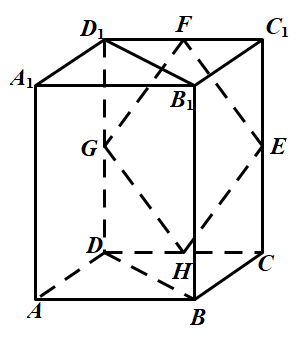
\includegraphics[width=24mm]{figs/js_image17.png}}\par\vspace{-1.0mm}\penalty10000
\lxopt{（注：请填上你认为正确的一个条件即可，不必考虑全部可能情况．）}
\begin{ansblock}[练-课时06-14]
% ans:练-课时06-14
\setlength{\anshang}{7.6mm}% 题14 起双位档（照答案册同值，块内局部）
\ansitem{14}{\(M\) 在线段 \(FH\) 上（例 \(M=F\)，答案不唯一）}
\end{ansblock}

\dangbadge{思}{维}{探}{索}

\tihao{15}\duoxuan\zu{K12 位置关系综合判定·文化载体多选（曲池）} \tieside{难}中国古代数学著作《九章算术》中，记载了一种称为“曲池”的几何体，该几何体的上下底面平行，且均为扇环形（扇环是指圆环被扇形截得的部分），现有一个如图所示的曲池，它的高为\(2\)，\(AA_1\)，\(BB_1\)，\(CC_1\)，\(DD_1\)均与曲池的底面垂直，底面扇环对应的两个圆的半径分别为\(1\)和\(2\)，对应的圆心角为\(90^{\circ}\)，则以下命题正确的是\nobreak(\kongwei)
\par\vspace{1.9mm}\penalty10000\noindent\makebox[\linewidth][c]{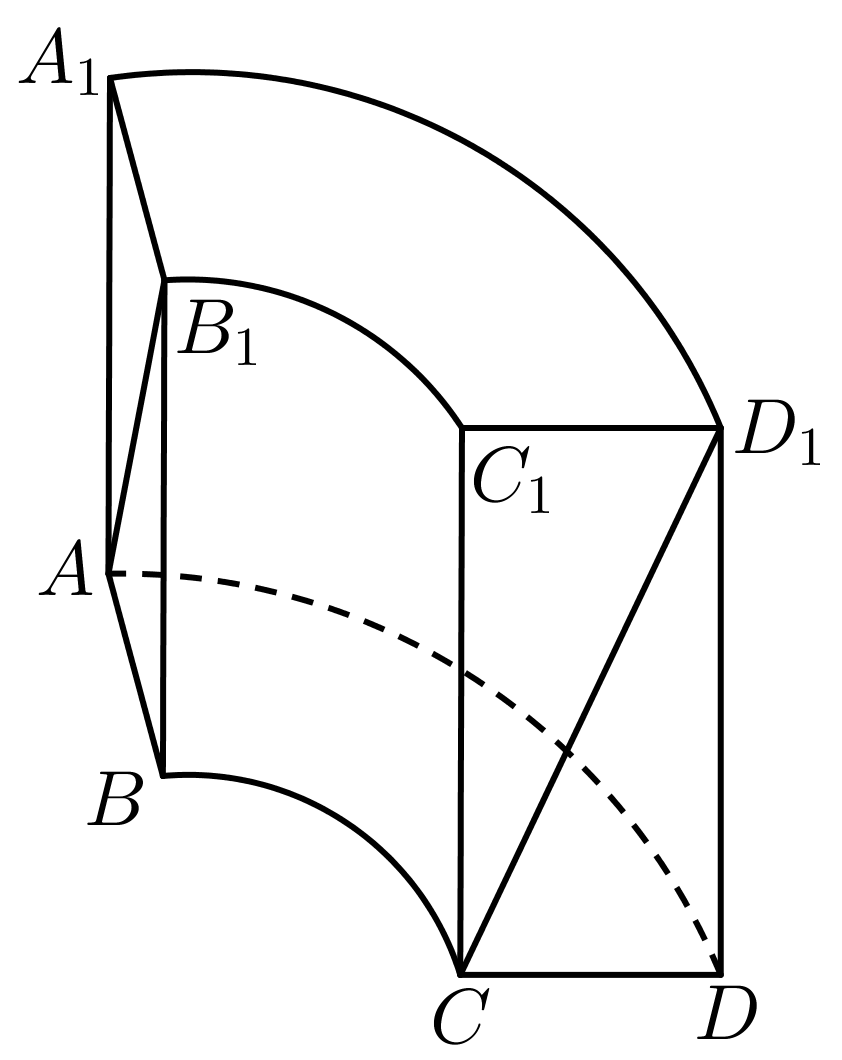
\includegraphics[width=30mm]{figs/js_image37.png}}\par\vspace{-1.0mm}\penalty-50
\lxopt{A．\(AB_1\)与\(CD_1\)成角的余弦值为\(\frac{4}{5}\)}
\lxopt{B．\(A_1\)，\(B\)，\(C\)，\(D_1\)四点不共面}
\lxopt{C．弧\(A_1D_1\)上存在一点\(E\)，使得\(BE\parallel CD_1\)}
\lxopt{D．以\(C\)点为球心，\(\sqrt{5}\)为半径的球面与曲池上底面的交线长为\(\frac{2}{3}\pi\)}
\begin{ansblock}[练-课时06-15]
% ans:练-课时06-15
\setlength{\anshang}{7.6mm}% 题15 起双位档（照答案册同值，块内局部）
\ansitem{15}{AD}
\end{ansblock}

\tihao{16}\zu{K13 公垂线段存在性判断（探究）} \tieside{难}已知长方体\(ABCD\text{-}\penalty100 A_1B_1C_1D_1\)中，\(AD=AB=2DD_1\)，判断满足下列条件的点\(M\)，\(N\)是否存在：\(M\in AD_1\)，\(N\in BD\)，\(MN\perp AD_1\)，\(MN\perp BD\)．
\xiexwei{20mm}
\begin{ansblock}[练-课时06-16]
% ans:练-课时06-16
\setlength{\anshang}{7.6mm}% 题16 起双位档（照答案册同值，块内局部）
\ansitem{16}{存在：\(\overrightarrow{AM}=\dfrac{2}{3}\overrightarrow{AD_{1}}\)、\(\overrightarrow{BN}=\dfrac{5}{6}\overrightarrow{BD}\)，\(|MN|=\dfrac{\sqrt{6}}{3}\)}
\end{ansblock}

\end{multicols}

\tailfill
\end{document}
